\subsection{TRADITIONAL HINDU COMPUTATIVE METHOD OF CHART COMPARISON
THE KUTA SYSTEM}
 

In this lesson we will examine an important method of computation for judging compatibility. It follows traditional approaches of Hindu Astrology and reflects aspects of Hindu culture. While the language may be difficult for us to understand, it can yield much useful information and is much simpler to do as we can simply look up the compatibility between different Nakshatras. Yet though this method is detailed, we must not rely upon it exclusively but rather use it in adjunct to the methods shown in the previous chapter. Generally speaking the influences on the seventh house and its lord will outweigh these elaborate calculations.

 

The traditional Indian method of judging compatibility included weighing different factors and giving them certain unit strengths. If the charts have a certain number of such points, they are regarded as good for relationship. If they fail to gain the required number, they are considered to be questionable for happy marriages. Most of these factors are based on the lunar constellations or Nakshatras, which we examine in more detail in Part III of the course. For the locations of the Nakshatras in the zodiac, please examine that section of the course.

 

While some factors in this method of computation appear strange at first, others follow obvious astrological principles. While we need not take each one of them too seriously in itself, the overall value they show can be an important index of compatibility. Yet such mechanical computation methods should not substitute for a more detailed chart analysis. They are a numerical short cut that is generally helpful but may not be enough in itself.

 

Below we examine how these factors are calculated. Yet you need not calculate the total yourself. All Vedic astrology software programs do this. They can also examine such positions from the Moon as well as the Ascendant, and compare the Kuta points overall between different charts.

 

 
\begin{figure}[H]
 \centering
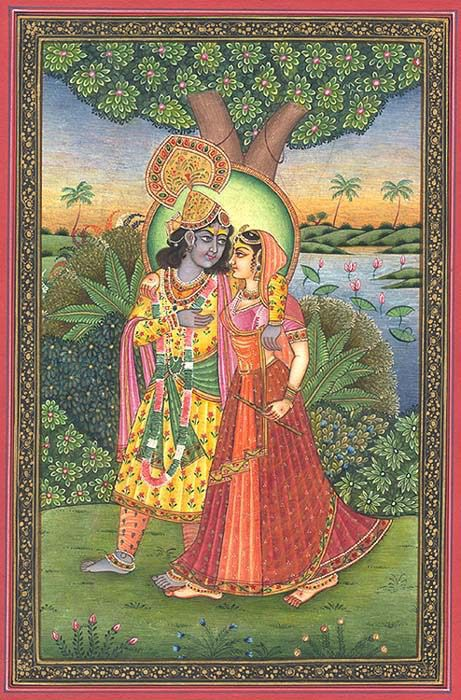
\includegraphics[width=0.8\textwidth]{pics/relationship1.png}
 \end{figure}

 

\subsubsection{1. DINA KUTA}
 

Count the Nakshatra of the man from that of the woman and divide the number by nine.
If the remainder is an even number: 0, 2, 4, 6, or 8, the result is good. If it is an odd number; 1, 3, 5, 7, 9, the result shows difficulties. Three units of compatibility are given if the result is good.
 

The idea is that the woman being feminine in nature should have a Nakshatra in a feminine (even numbered) relationship from that of the man.

 

\subsubsection{2. GANA KUTA}
 

The Nakshatras are classified into three temperaments or energy types (gana) as Deva (divine), Manusha (human) or Rakshasa (demonic). They generally correspond to sattvic, rajasic and tamasic qualities. They also have an energetic effect.

 

Deva or divine Nakshatras are characterized by faith, openness, loyalty and devotion, which however, may be conservative or superficial.
Manusha or human Nakshatras are characterized by change, turbulence and uncertainty, which however, may be progressive.
Rakshasa Nakshatras are characterized by negation, independence, eccentricity, and harsh actions, which however may lead a person to break through attachments or conventions.
 

These groups do not of themselves make the individuals born under them of higher or lower spiritual nature. That comes from the chart as a whole.

 

Generally, one should marry a person of the same Gana. It is also considered that a Rakshasa man can marry a Deva or Manusha girl, but that a Deva or Manusha man should not marry a Rakshasa girl. These Ganas are as follows:

 

DEVA GANAS are Ashvini, Mrigashira, Punarvasu, Pushya, Hasta, Svati, Anuradha, Shravana, and Revati.
MANUSHA GANAS are Bharani, Rohini, Ardra, Purva Phalguni, Uttara Phalguni, Purvashadha, Uttarashadha, Purva Bhadra, and Uttara Bhadra.
RAKSHASA GANAS are Krittika, Aslesha, Magha, Chitra, Vishakha, Jyeshta, Mula, Dhanishta and Shatabhishak.
 

This factor counts for six units. Some astrologers say that if the Nakshatra of the woman is more than 14th from the man, this problem can be ignored.

 

We also note that Deva Nakshatras are good Moons under which to proceed with any favorable actions. Manusha are moderate, and Rakshasa are usually not recommended. We can note their effects under the section of Part III on Astrological Forecasting Part 1, to see their nature and results.

 

\subsubsection{3. MAHENDRA}
 

It is good if the Nakshatra of the man is 4th, 7th, 10th, 13th, 16th, 19th, 22nd or 25th from that of the woman.

 

\subsubsection{4. STRI DIRGHA}
 

The Nakshatra of the male should be at least nine away from that of the female. By some accounts seven is enough. The idea is that some distance between the Moons is helpful for compatibility. This consideration can be ignored if Rashi Kuti (factor 6) or Graha Maitri (factor 7) prevail.

 

\subsubsection{5. YONI KUTA}
 

This is perhaps the strangest factor of compatibility in Vedic Astrology. It divides the Nakshatras into several animal types, said to represent their sexual organs. It is thought to measure sexual compatibility between the partners.

 

\subsubsection{NAKSHATRAS AND RULING ANIMALS}

\begin{center}
\begin{tabular}{ l l l l}

 NAKSHATRAS              & ANIMAL             &SEX \\

1.    ASHWINI	&HORSE	&MALE.                             \\
2.    BHARANI	&ELEPHANT	&MALE.                      \\
3.    KRITTIKA	&SHEEP	&FEMALE                           \\
4.    ROHINI	&SERPENT	&MALE                         \\
5.    MRIGASHIRAS	&SERPENT	&FEMALE                         \\
6.    ARDRA	&DOG	&FEMALE                         \\
7.    PUNARVASU	&CAT	&FEMALE                         \\
8.    PUSHYA	&SHEEP	&MALE                         \\
9.    ASHLESHA	&CAT	&MALE                         \\
10.  MAGHA	&RAT	&MALE                         \\
11.  PURVA PHALGUNI	&RAT	&FEMALE                         \\
12.  UTTARA PHALGUNI	&COW	&MALE                         \\
13.  HASTA	&BUFFALO	&FEMALE                         \\
14.  CHITRA	&TIGER	&FEMALE                         \\
15.  SWATI	&BUFFALO	&MALE                         \\
16.  VISHAKHA	&TIGER	&MALE                         \\
17.  ANURADHA	&RABBIT	&FEMALE                         \\
18.  JYESHTA	&RABBIT	&MALE                         \\
19.  MULA	&DOG	&MALE                         \\
20.  PURVASHADHA	&MONKEY	&MALE                         \\
21.  UTTARASHADHA	&MONGOOSE	&MALE                         \\
22.  SHRAVANA	&MONKEY	&FEMALE                         \\
23.  DHANISHTA	&LION	&FEMALE                         \\
24.  SHATABHISHAK	&HORSE	&FEMALE                         \\
25.  PURVA BHADRA	&LION	&MALE                         \\
26.  UTTARA BHADRA	&COW	&FEMALE                         \\
27.  REVATI	&ELEPHANT	&FEMALE                         \\
 
 \end{tabular}
\end{center}
 

\subsubsection{HOSTILE OR INCOMPATIBLE ANIMALS}

 

These are the horse and buffalo, elephant and lion, sheep and monkey, serpent and mongoose, dog and rabbit, cat and rat, cow and tiger. Combinations of these should be avoided in marriage. Generally, this is enough to reject a marriage according to this system. This gives 0 points in terms of Yoni Kuta.

 

\subsubsubsection{UNFRIENDLY ANIMALS}

HORSE	cow, tiger, lion	ELEPHANT	tiger
SHEEP	dog, rat, tiger, lion	SERPENT	cat, rat, cow, buffalo
DOG	sheep, rat, tiger, mongoose, lion	CAT	serpent, tiger, mongoose, lion
RAT	sheep, serpent, dog, mongoose	COW	horse, serpent, lion
BUFFALO	Serpent, tiger, lion	TIGER	horse, elephant, sheep, dog, cat, buffalo, rabbit, monkey, lion
RABBIT	Horse, tiger, lion	MONKEY	tiger
MONGOOSE	Dog, rat	LION	horse, sheep, dog, cat, cow, tiger, rabbit.
 

These are counted from the Nakshatra of the male. Marriage between unfriendly animals is considered to be more difficult. They give 1 point in terms of Yoni Kuta.

 

\subsubsubsection{NEUTRAL ANIMALS}

HORSE	Elephant, sheep, dog, cat, mongoose	ELEPHANT	sheep, serpent, buffalo, monkey
SHEEP	Elephant, cow, buffalo, mongoose	SERPENT	horse, elephant
DOG	Horse, elephant, serpent, cat, cow, buffalo, monkey	CAT	horse, elephant, sheep, dog, cow, buffalo, mongoose
RAT	Horse, elephant, cow, buffalo, tiger, rabbit, monkey, lion	COW	elephant, dog, cat, rat, monkey, mongoose
BUFFALO	Dog, cat, rat, rabbit, monkey, mongoose	TIGER	serpent, rat, mongoose
RABBIT	Elephant, sheep, serpent, rat, buffalo, monkey, mongoose	MONKEY	serpent, dog, rat, cow, buffalo, rabbit, lion
MONGOOSE	Horse, elephant, cat, cow, buffalo, tiger, rabbit, lion	LION	serpent, rat, buffalo, monkey, mongoose
 

These are considered average in terms of compatibility. They give 2 points in terms of Yoni Kuta.

 

\subsubsubsection{FRIENDLY ANIMALS}

HORSE	serpent, rabbit and monkey	ELEPHANT	sheep, serpent, buffalo and monkey
SHEEP	elephant, cow, buffalo and mongoose	SERPENT	horse, elephant
DOG	None	CAT	rabbit, monkey
RAT	None	COW	sheep, buffalo, rabbit
BUFFALO	elephant, sheep, cow	TIGER	none
RABBIT	cat, cow	MONKEY	horse, elephant, cat, mongoose
MONGOOSE	sheep, monkey	LION,	none
 

These relationships are also determined from the Nakshatra of the male. Hence, a man under the horse will generally do well with a woman under the serpent, as there is friendship between their animals. These give 3 points in terms of Yoni Kuta.

 

\subsubsubsection{SAME ANIMAL}

 

Marriage between men and women of the same animal is considered to be the best, particularly if they are of male and female stars respectively, for example, an Ashwini man and a Shatabhishak woman. It is conducive to sexual compatibility and happiness through children. Relationships of the same animal give 4 points in terms of Yoni Kuta.

 

Some animal types are difficult in terms of sexual compatibility. Such are, in order of difficulty, the tiger, lion, dog and rat, which have no friendly animals. Those of these animal types have more difficulty in sexual relationships. The serpent, cat and rabbit have some difficulties as well. Most generally compatible are the monkey and elephant. The others fall in the middle.

 

In addition, it is more favorable if the males animal falls in a masculine division and if the womans animal falls in a feminine division. Please note the table at the end of this lesson, which allows you to look up the compatibility numbers between various Nakshatras based upon this principle.

 
\begin{figure}[H]
 \centering
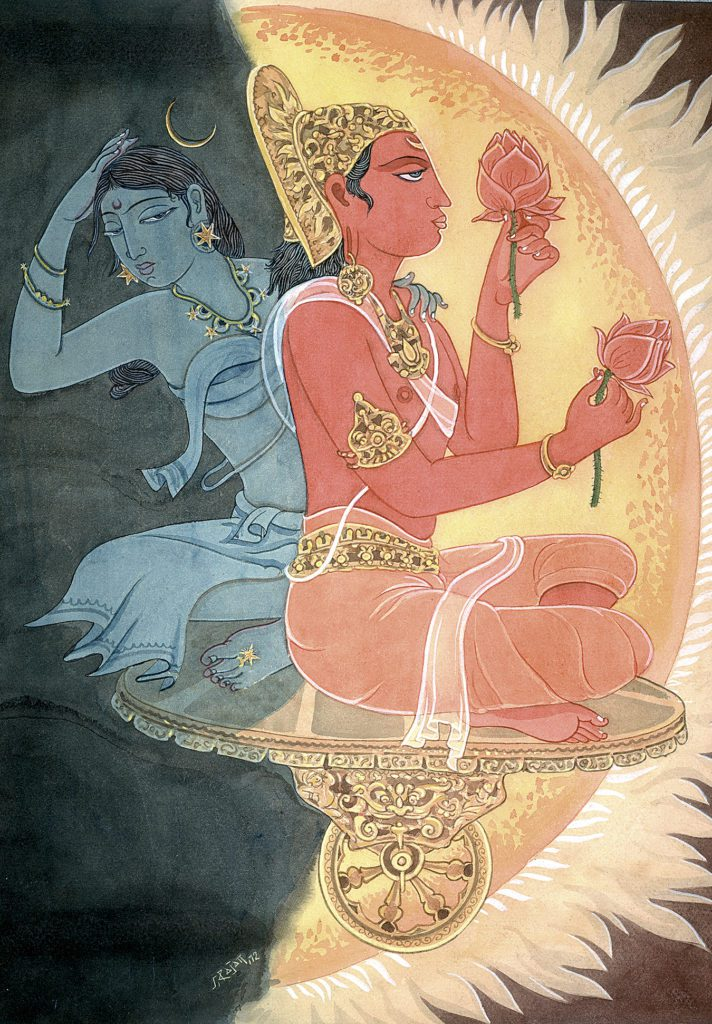
\includegraphics[width=0.8\textwidth]{pics/relationship2.png}
\caption{Lord Shiva and Parvati Devi}
 \end{figure}




\subsubsection{6. RASHI KUTA}
 

This refers to the relationship between the Moon signs (Chandra Rashis) in the birthchart, which is obviously an important consideration in all astrological compatibility examinations. Vedic Astrology gives us a system to compute this relationship.

 

If the Moon sign of the male is SECOND from the female, and hers is twelfth from his, it is not considered good. For example, if the male has the Moon in Virgo and the female has it in Leo. On the other hand, if the males Moon is twelfth from the female, it is considered good, ie. if his is in Leo and hers is in Virgo.

 

If the Moon sign of the male is THIRD from the female, this gives difficulty and sorrow, but if the Moon sign of the female is third from the male, this gives ease and happiness.
If the Moon sign of the male is FOURTH from the female, this is said to give poverty, but if the Moon sign of the female is fourth from the male, this is said to give wealth.
If the Moon sign of the male is FIFTH from the female, this is said to give unhappiness, while if her Moon sign is fifth from his it is said to give joy.
If his Moon sign is SIXTH from hers it causes difficulty to children but if hers is sixth from his, it gives happiness through children.
If the Moon signs are SEVENTH or opposite each other this is best. It gives mutual health and happiness. Moons opposite each other give balance and capacity for communication.
 

The general logic of this sequence is that it is better for the mans Moon to be placed before the womans Moon in the zodiac. As planets cast their aspects forwards in the zodiac, this gives the males chart the lead in action, which is in harmony with the nature of masculine energy. If the females Nakshatra is before in the zodiac, this can make her dominant over him.

 

If the Moon sign is the same for both partners, the Nakshatra in which the Moon is located should be different. That of the male should be before that of the female. For example, if both have Aries Moons, it is better if the mans Moon is in Ashwini, which is in early Aries, and the womans is in Bharani, which is in later Aries. However, in the actual total Kuta system, the same Moon sign is generally good whether the Nakshatra of the male is before or after that of the female.
If the Nakshatra is also the same for both partners this is considered GOOD in the case of Rohini, Ardra, Magha, Hasta, Vishakha, Shravana, Uttara Bhadra, and Revati.
It is considered AVERAGE if the Nakshatras are Ashvini, Krittika, Mrigashiras, Punarvasu, Pushya, Purva Phalguni, Uttara Phalguni, Chitra, Anuradha, Purvashadha and Uttarashadha.
It is considered NOT GOOD and not recommended in the case of Bharani, Ashlesha, Svati, Jyeshta, Mula, Dhanishta, Shatabhishak and Purva Bhadra.
 

Some astrologers consider that it is all right if the birth Nakshatra is the same if the Moons are located in different quarters within the Nakshatra. In regard to Shatabhishak, Hasta, Swati, Ashwini, Krittika, Purvashadha, Mrigashiras and Magha, it is considered all right if both partners are born in the first quarter of the Nakshatra.

 

This factor has 7 units and so is weighted fairly strongly. However, we might want to consider it in more detail. What is being weighed is the relationship between the Moon signs or the Moon to Moon relationship. For this, we can go back to the first section on Relationship and examine the relationship between Moons in the chart as a whole.

 

\subsubsection{7. GRAHA MAITRAM}
 

This refers to the relationship between the lords of the Moon signs in terms of friendship or enmity. Some astrologers count this only in terms of natural friendship, others consider the temporal as well. I am inclined to the latter opinion.

 

For example, if the mans Moon is in Pisces ruled by Jupiter and the womans Moon is in Aries ruled by Mars, then their Moon lords are natural friends.

 

When the planets involved are both friends, this factor is obtained in full. When one is a friend and the other is neutral, it is still good. When both are neutral it is only average or passable. When one is neutral and the other is inimical, it is difficult. When both are enemies, this factor of compatibility does not exist.

 

When this factor is not present in the Moons sign, it is sometimes looked for in the Moons Navamsha. This factor counts for 5 units. To determine this, we have to look at each chart separately.

 

\subsubsection{8. VASHYA KUTA}
 

The Moon sign gains power to influence or control other signs, which is referred to here. These are for:

 

Aries – Leo and Scorpio.
Taurus – Cancer and Libra.
Gemini – Virgo.
Cancer – Scorpio and Sagittarius
Leo – Libra
Virgo – Pisces and Gemini
Libra – Capricorn and Virgo
Scorpio – Cancer
Sagittarius – Pisces
Capricorn – Aries and Aquarius
Aquarius – Aries
Pisces – Capricorn
 

We see that a few signs are mutually influencing. These are Gemini and Virgo, Cancer and Scorpio. This factor counts for two kuta points.

 

\subsubsection{9. RAJJU KUTA}
 

Rajju means rope. It shows possibilities of misfortune in married life. The Nakshatras are divided into five groups based upon this factor. This factor counts for four points.

 

FOOT– Padarajju
Ashvini, Ashlesha, Magha, Jyeshta, Mula, Revati
HIP– Katirajju
Bharani, Pushya, Purva Phalguni, Anuradha, Purvashadha, Uttara Bhadra
NAVEL– Udararajju
Krittika, Punarvasu, Uttara Phalguni, Vishakha, Uttarashadha, Purva Bhadra
THROAT– Kantharajju
Rohini, Ardra, Hasta, Swati, Shravana, Shatabhishak
HEAD – Shirorajju
Dhanishta, Chitra, Mrigashira
 

The Nakshatras wherein the Moon is located should not fall in the same Rajju for male and female. If they both occur in the head, the husbands longevity may be threatened. If they both occur in the throat, the wifes longevity may be threatened. If they both occur in the stomach, the childrens longevity may be threatened. If they both occur in the navel, there may be poverty. If they both occur in the hip, the couple may have to always be wandering.

 

\subsubsection{10. VEDHA/ INCOMPATIBLE NAKSHATRAS}
 

Each Nakshatra has one that it particularly afflicts and with which it is therefore generally incompatible. It is best for those of these conflicting Nakshatras not to marry each other. This factor counts for two points. These are:

 

1. Ashwini and 18. Jyeshta	2. Bharani and 17. Anuradha
3. Krittika and 16. Vishakha	4. Rohini and 15. Swati
5. Mrigashira and 23. Dhanishta	6. Ardra and 22. Shravana
7. Punarvasu and 21. Uttarashadha	8. Pushya and 20. Purvashadha
9. Ashlesha and 19. Mula	10. Magha and 27. Revati
11. Purva Phalguni and 26. Uttara Bhadra	12. Uttara Phalguni and 25. Purva Bhadra
13. Hasta and 24. Shatabhishak.	14. Chitra, no incompatible Nakshatras
 

 

\subsubsection{11. VARNA/ CLASS}
 

The lunar signs are divided into four groups based upon class or varna. Brahmin is the spiritual class or those of knowledge, Kshatriya the nobility or people of honor, Vaishya the merchants or commercial people, and Shudra, the servant or labor class. They tend to represent our temperament and values, but are only very vague indications of these that should not be taken too seriously. These are:

 

 BRAHMIN	 water signs	 Cancer, Scorpio, Pisces
 KSHATRIYA	 fire signs	 Aries, Leo, Sagittarius
 VAISHYA	 air signs	  Gemini, Libra, Aquarius
 SHUDRA	 earth signs	 Taurus, Virgo, Capricorn
 

The unit of agreement here is only 1 point. This we might add, however, is an extremely important factor to consider, namely spiritual compatibility. However, the method of calculating it here is very approximate and rarely accurate. It is better to use other more complex and accurate methods of judging spiritual types.

 

\subsubsection{12. NADI KUTA}
 

This is an attempt to compute the physical type according to the three Ayurvedic doshas. By this system, individuals of the same doshic type should not marry, as they will increase the factors of disease in each other. Each of the Nakshatras is assigned one of them.

 

VATA
Ashvini, Ardra, Punarvasu, Uttara Phalguni, Hasta, Jyeshta, Mula, Shatabhishak, Purva Bhadra
PITTA
Bharani, Mrigashiras, Pushya, Purva Phalguni, Chitra, Anuradha, Purvashadha, Dhanishta, Uttara Bhadra
KAPHA
Krittika, Rohini, Ashlesha, Magha, Swati, Vishakha, Uttarashadha, Shravana, Revati
 

If Nadi Kuta is not present, it can be counted on the quarters of the Nakshatras. If it is present there, that can also be helpful. This factor is given 8 units. However, we should note that it is only approximate. The Nakshatra in itself is not always enough to determine constitutional type. Hence, if we have another way of determining it, we should resort to that instead.

 

\subsubsection{SUMMARY}

 

In summary, we note that the factors examined in this system are important but the way in which some of them are gauged is not beyond question. Perhaps this system may have to be revised relative to modern conditions. However, it is still very helpful and all Vedic astrologers should know how to use it, particularly if they will be dealing with Indian clients.

 

Please look up the Kuta or chart compatibility on your Vedic software system.  Compare the star or Nakshatra of the male partner (bridegroom) with the female partner (bride). This gives a general compatibility rating considering most of the points of the computative method.

 

Good compatibility is usually above 20 points, though as little as 18 can be all right and is average. High compatibility is above 25 points. Low compatibility is below 15 points. Below 10 can be very difficult.

 

While in India this method is taken very seriously, here I dont think we can follow it rigidly. I have seen at least some successful or enduring marriages with less than 15 points of compatibility. I have also seen some divorces with more than 25 points. It is obvious that based on Nakshatra alone there will be many people that we will be compatible with in terms of this method alone.

 

\subsubsection{MEANING OF THE KUTA SYSTEM}

 

This system measures primarily the compatibility between the Moons and Nakshatras. This is very important because the Moon shows emotional affinity and the ability to function together as a family. However, a good Moon relationship is not enough for a successful relationship. And relationships can be successful without good Moon relationships if Venus and Jupiter are favorably placed between the charts.

 

When the Moons are favorable, we feel good around one another, our moods harmonize, and we do not feel invaded or threatened by the other persons presence in our lives. When the Moons are unfavorable, it may be difficult to trust the other person, or to feel that we can be ourselves around them. They are much more likely to seem foreign, alien or different from us.

 

Therefore, it is best to use the computative method along with the comparative method, considering the overall nature of the charts involved. By itself the Kuta system can cause us to make hasty or superficial judgments. Usually if the points are high, that is good, if the charts are otherwise in harmony. If the points are low, that can be counteracted (unless the total points is very low, like below 10) if the charts are otherwise in harmony. If the points are high and the charts are otherwise disharmonious, it will not be sufficient for a good relationship. If the points are low but the charts are otherwise harmonious, it may be sufficient for a good relationship.

 

Generally speaking, there is little that can counteract the effects of a bad seventh house in the chart, while there is little that can damage a good seventh house in the chart. Please remember this point.

 

We should first examine the computative method, as it is quick to note, and then go into comparative analysis for a more clear decision on the matter.
We have also included for easy computation, a chart of the Yoni Kuta.
 



 

\subsubsection{ASTROLOGY AND RELATIONSHIP COUNSELING}

 

Astrology is a helpful tool in relationship counseling because it reveals the energetic issues behind relationships. It can help each person see their partners view of the world, which is usually not the same as their own. It can also help show the factors of projection – what we are imagining about the partner – which may not be their nature and must eventually cause problems. Sometimes we may be relating to one planetary influence in another person but not the others.

 

Yet relationship counseling can be difficult, particularly for clients having trouble in their relationships with each other, for those seeking divorce, or if one partner is trying to use the reading to get the other partner into or out of a marriage. For this reason, we recommend doing individual readings before doing readings for couples. It is easiest to do a compatibility reading if the relationship is just beginning and no major commitments and attachments have been formed. If the relationship is already established, we might want to orient the reading more toward helping the couple understand each other, rather than telling them if they are really compatible in the long run. Hence, a certain amount of discretion may be required, even the charts do not look good together.

 

This is the easiest area of astrological counseling where we can offend or upset other people, even if we are right. The important thing is to give the client advice that they are able to use.

 

These relationship issues have been mainly oriented toward male-female or marriage relationships. However, they apply to some extent to all human relationships. People with whom we have disharmonious Moons are likely to be trouble to work with or be friends with. Other relationship incompatibilities, whether judged by the comparative or computative methods, can yield similar problems. Hence, if we have an associate that it is particularly easy or particularly difficult to be with, it can help to examine the charts to see what the conflicting patterns may be.

 

Even as astrologers we can be aware of these patterns. For example, I have Mars in Scorpio in my birthchart. Hence I understand that clients with the Moon in Scorpion are more likely to feel criticized, hurt or even offended by what I may say because of the effect of Mars on the Moon. With them I am inclined to be particularly sensitive to avoid hurting their feelings even on minor issues.